\documentclass[12.5pt]{article}
\usepackage{graphicx} % Required for inserting images
\usepackage{epigraph}
\usepackage{geometry}
\usepackage{setspace} % Add the setspace package
\usepackage{titlesec} % Add the titlesec package for customizing titles

% Optional: customize the style of epigraphs
\setlength{\epigraphwidth}{0.5\textwidth} % Adjust the width of the epigraph
\renewcommand{\epigraphflush}{flushright} % Align the epigraph to the right
\renewcommand{\epigraphrule}{0pt} % No horizontal rule
\usepackage[most]{tcolorbox}
\usepackage{amsmath, amssymb, amsthm}
\usepackage{graphicx}
\usepackage[utf8]{inputenc}
\usepackage{hyperref} % Added for hyperlinks
\usepackage{listings} % Added for code listings
\usepackage{color}    % Added for color definitions
\usepackage[super]{nth}
\usepackage{fancyhdr}
\usepackage{tikz}
\usepackage{cite}
\usepackage{algpseudocode}
\usepackage{subcaption}
\usepackage{cleveref}
\usepackage[font=small]{caption}
\usetikzlibrary{shapes.geometric, arrows, positioning}
\usepackage{dirtree}

\tikzstyle{startstop} = [rectangle, rounded corners, text centered, draw=black, fill=red!30]
\tikzstyle{io} = [trapezium, trapezium left angle=70, trapezium right angle=110, text centered, draw=black, fill=blue!30]
\tikzstyle{process} = [rectangle, text centered, draw=black, fill=orange!30]
\tikzstyle{decision} = [diamond, text centered, draw=black, fill=green!30]
\tikzstyle{arrow} = [thick,->,>=stealth]

% Define the header and footer for general pages
\pagestyle{fancy}
\fancyhf{} % Clear all header and footer fields
\fancyhead{} % Initially, the header is empty
\fancyfoot[C]{\thepage} % Page number at the center of the footer
\renewcommand{\headrulewidth}{0pt} % No header line on the first page of chapters
\renewcommand{\footrulewidth}{0pt} % No footer line

% Define the plain page style for chapter starting pages
\fancypagestyle{plain}{%
  \fancyhf{} % Clear all header and footer fields
  \fancyfoot[C]{\thepage} % Page number at the center of the footer
  \renewcommand{\headrulewidth}{0pt} % No header line
}


% Redefine the 'plain' style for the first page of chapters
\fancypagestyle{plain}{%
  \fancyhf{}%
  \fancyfoot[C]{\thepage}%
  \renewcommand{\headrulewidth}{0pt}%
}

% Header settings for normal pages (not the first page of a chapter)
\fancyhead[L]{\slshape \nouppercase{\leftmark}} % Chapter title in the header
\renewcommand{\headrulewidth}{0.4pt} % Header line width on normal pages

\setlength{\headheight}{12pt}

% Define colors for code listings
\definecolor{codegreen}{rgb}{0,0.6,0}
\definecolor{codegray}{rgb}{0.5,0.5,0.5}
\definecolor{codepurple}{rgb}{0.58,0,0.82}
\definecolor{backcolour}{rgb}{0.95,0.95,0.92}

% Setup for code listings
\lstdefinestyle{mystyle}{
    backgroundcolor=\color{backcolour},
    commentstyle=\color{codegreen},
    keywordstyle=\color{magenta},
    numberstyle=\tiny\color{codegray},
    stringstyle=\color{codepurple},
    basicstyle=\ttfamily\footnotesize,
    breakatwhitespace=false,
    breaklines=true,
    captionpos=b,
    keepspaces=true,
    numbers=left,
    numbersep=5pt,
    showspaces=false,
    showstringspaces=false,
    showtabs=false,
    tabsize=2
}

\lstset{style=mystyle}

% Definition of the tcolorbox for definitions
\newtcolorbox{definitionbox}[1]{
  colback=red!5!white,
  colframe=red!75!black,
  colbacktitle=red!85!black,
  title=#1,
  fonttitle=\bfseries,
  enhanced,
  breakable,
}

% Definition of the tcolorbox for remarks
\newtcolorbox{remarkbox}[1]{
  colback=blue!5!white,     % Light blue background
  colframe=blue!75!black,   % Darker blue frame
  colbacktitle=blue!85!black, % Even darker blue for the title background
  title=#1,            % Title text for remark box
  fonttitle=\bfseries,      % Bold title font
  enhanced,
  breakable,
}

% Definition of the tcolorbox for examples
\newtcolorbox{examplebox}[1]{
  colback=green!5!white,    % Light green background
  colframe=green!75!black,   % Darker green frame
  colbacktitle=green!85!black,  % Even darker green for the title background
  title=#1,         % Title text for example box
  fonttitle=\bfseries,    % Bold title font
  enhanced,
  breakable,
}

% Definitions and examples will be put in these environments
\newenvironment{definition}
    {\begin{definitionbox}}
    {\end{definitionbox}}

\newenvironment{example}
    {\begin{examplebox}}
    {\end{examplebox}}

\onehalfspacing

\geometry{top=1.5in} % Adjust the value as needed

% Customization for chapter titles
\titleformat{\chapter}[display] % Use 'display' to put number and title on separate lines
  {\normalfont\LARGE\bfseries} % Format for the chapter title
  {Chapter \thechapter} % Display "Chapter X"
  {0.5em} % Space between "Chapter X" and the title
  {\Huge} % Chapter title format
\titlespacing*{\chapter}{0pt}{-15pt}{15pt} % Adjust spacing around chapter title
\pagestyle{plain}


\title{C1 Report}
\author{Ngoc Anh Doan}
\date{December 2024}

\begin{document}

\maketitle
\newpage
\begin{center}
    \textbf{Introduction}
\end{center}
In this coursework, the aim is to develop a Python package, \texttt{dual\_autodiff}, that performs automatic differentiation using dual numbers. The coursework involves constructing a robust software package that can compute derivatives efficiently in forward-mode, a fundamental approach for various applications such as deep learning and optimization. By leveraging the properties of dual numbers, the package will implement essential operations, mathematical functions, and derivative computations. Additionally, this coursework emphasizes best practices in software development, including project packaging, testing, documentation, and optimizing performance through Cython.

Through this coursework, the theoretical underpinnings of dual numbers will be explored, demonstrated their practical implementation, and analyzed performance differences between Python and Cython-based solutions. The final deliverable include a comprehensive repository featuring a working package, tests, documentation, and a comparison of numerical and analytical derivative methods.

\begin{center}
\textbf{Declaration of AI Assistance}
\end{center}
In this coursework, I use ChatGPT, a language model developed by OpenAI, as a supportive tool for specific tasks. ChatGPT was employed to:
\begin{enumerate}
    \item Debug Code: Identify and resolve issues in code implementations.
    \item LaTex help: Provide suggestions for improving better display and use of LaTex.
\end{enumerate}

The use of ChatGPT was restricted to enhance understanding, solving programming-related challenges, and improving the clarity of implementation. All decisions regarding the final design, implementation, and analysis were independently verified and made by me. ChatGPT's assistance was supplementary and did not generate or replace original work or intellectual contributions in this coursework.

All the files were run on Macbook Air M1 2020, Python version 3.9.

\newpage
\section{Create project repository structure and configuration 
\newline(task 1+2)}

\subsection{Directory Structure}\label{1.1}
The project directory was carefully structured to ensure simplicity, usability, and clarity. A Python package named \texttt{dual\_autodiff} was created, adhering to software engineering best practices, including the organization of source code, tests, and documentation.

The directory structure is as follows:

\dirtree{%
    .1 dual\_autodiff/.     
    .2 dual\_autodiff/. 
    .3 \_\_init\_\_.py. % Makes it a Python package.
    .3 dual.py. % Main implementation of dual numbers.
    .3 tests/. % Unit tests.
    .2 docs/. % Documentation.
    .3 conf.py. % Configuration file for Sphinx.
    .3 index.rst. % Main documentation file.
    .3 .... % Other documentation files.
    .2 pyproject.toml. % Project configuration file.
    .2 README.md. % Project description and instructions.
    .2 .gitignore.
    .2 LICENSE. % Licensing information.
}
The rigorous organization of the project guarantee ease of use, but also easier management and extension of the package. A test folder is used, ensure all functionalities are thoroughly verified. The report elaborates \texttt{test} and \texttt{doc} in a deeper level in the next tasks.

\subsection{Key Files and Their Purposes} 
This section details the files contained in the repository and what their uses are.
\begin{itemize}
    \item \textbf{\texttt{dual\_autodiff/}}: Contains the source code to make the package.
    \begin{itemize}
        \item \texttt{dual.py}: Implements the \texttt{Dual} class and the operations for dual numbers.
        \item \texttt{\_\_init\_\_.py}: Allows importing \texttt{dual\_autodiff} as a package.
        \item \textbf{\texttt{tests/}}: Contains all unit tests.
    \end{itemize}
    \item \textbf{\texttt{docs/}}: Stores the project's documentation.
    \item \textbf{\texttt{pyproject.toml}}:
    \begin{itemize}
        \item Replaces \texttt{setup.py} for project configuration in this project.
        \item Includes metadata (author, version, dependencies) and build instructions.
    \end{itemize}
    \item \textbf{\texttt{README.md}}: Provides an overview of the project, installation instructions, and usage examples.
    \item \textbf{\texttt{.gitignore}}: Ensures unnecessary or sensitive files (e.g., \texttt{.pyc}, \texttt{\_\_pycache\_\_}) are not included in version control.
    \item \textbf{\texttt{LICENSE}}: Specifies the open-source license for the project.
\end{itemize}

\subsection{Project Configuration with \texttt{pyproject.toml}}
The \texttt{pyproject.toml} file was created adhering to Python's best practices \cite{WinNT}. It standardizes project metadata, dependencies, and build system settings, replacing older tools like \texttt{setup.py} for many tasks. It has the following contents: 
\begin{verbatim}
[build-system]
requires = ["setuptools>=61.0", "wheel", "setuptools_scm", "cython"]
build-backend = "setuptools.build_meta"

[project]
name = "dual_autodiff"
version = "0.1.0"
description = "Automatic differentiation using dual numbers."
readme = "README.md"
authors = [
    { name = "Ngoc Anh Doan", email = "nad60@cam.ac.uk" }
]
license = { file = "LICENSE" }
keywords = ["automatic-differentiation", "dual-numbers", "forward-mode"]
classifiers = [
    "Programming Language :: Python :: 3",
    "Operating System :: OS Independent",
    "License :: OSI Approved :: MIT License"
]
dependencies = [
    "numpy"
]
[tool.setuptools.packages.find]
where = ["dual_autodiff/"]
\end{verbatim}

The \texttt{pyproject.toml} file serves as the central configuration for the project, contains several key sections:

The \texttt{[build-system]} section specifies the build system requirements, including tools like \texttt{setuptools}, \texttt{wheel}, \texttt{setuptools\_scm} (for versioning), and \texttt{cython} (for performance optimization and later package cythonization). The \texttt{build-backend} is set to \texttt{"setuptools.build\_meta"}, instructing tools like \texttt{pip} on how to build the package.

The \texttt{[project]} section includes essential metadata about the package. This encompasses the \texttt{name} (a unique identifier for PyPI), the \texttt{version} (initial release version), a short \texttt{description} of the package's purpose, and the \texttt{readme}, which points to the \texttt{README.md} file for long-form project descriptions. Additionally, the \texttt{authors} field lists the author's name and contact email, while the \texttt{license} field specifies the license file, such as the MIT license. The \texttt{keywords} field improves searchability on PyPI, and the \texttt{classifiers} categorize the project for better visibility and indexing.

The \texttt{[dependencies]} section lists the required dependencies to use the package, such as \texttt{numpy} in this case.

Finally, the \texttt{[tool.setuptools.packages.find]} section configures \texttt{setuptools} to locate the Python package files. It ensures that all relevant files within the \texttt{dual\_autodiff/} directory are included in the final distribution. This structure ensures clarity, maintainability, and compatibility with modern Python packaging tools.

\newpage
\section{Dual Package (task 3+4)}
\subsection{Setting Up Dual}

\subsection*{Definition of Dual Numbers}
A dual number \cite{dualdef} is any number which can be expressed as:
\[
x = a + b\epsilon
\]
where:
\begin{itemize}
    \item \( a \): The real part of the dual number.
    \item \( b \): The dual part, representing derivative information.
    \item \( \epsilon \): An infinitesimal number satisfying \( \epsilon^2 = 0 \).
\end{itemize}

This formulation enables dual numbers to represent both function values and their derivatives, making them particularly useful for automatic differentiation.

\subsection*{Implementation}\label{2.1}

The \texttt{Dual} class is initialised with two components: \texttt{real} and \texttt{dual}. The class is designed to handle both the value of a function and its derivative simultaneously.

\begin{lstlisting}[language=Python]
class Dual:
    __slots__ = ['real', 'dual']

    def __init__(self, real: float, dual: float = 0.0):
        self.real = real
        self.dual = dual
        
#Example: 
x = Dual(5, 18)
print(x.real, x.dual)

# and then we can get the expected output:
5, 18
\end{lstlisting}

The \texttt{\_\_slots\_\_} attribute optimises memory usage and improves performance by explicitly declaring the class \texttt{Dual} can only have two attributes \texttt{real} and \texttt{dual}. \cite{slot}


\subsection{Mathematical Operations}

\subsubsection{Arithmetic Operations}
The basic arithmetic operations on dual numbers \( x = a + b\epsilon \) and \( y = c + d\epsilon \) can be defined as follow:

\begin{itemize}
    \item \textbf{Addition}:
    \((a + b\epsilon) + (c + d\epsilon) = (a + c) + (b + d)\epsilon\)
    \item \textbf{Subtraction}:
    \((a + b\epsilon) - (c + d\epsilon) = (a - c) + (b - d)\epsilon\)
    \item \textbf{Multiplication}:
    \((a + b\epsilon) \cdot (c + d\epsilon) = (a \cdot c) + (a \cdot d + b \cdot c)\epsilon\)
    \item \textbf{Division}:
    \[
    \frac{(a + b\epsilon)}{(c + d\epsilon)} = \frac{a}{c} + \frac{b \cdot c - a \cdot d}{c^2}\epsilon \quad \text{(for \( c \neq 0 \))}.
    \]
\end{itemize}

We can have a look at an example of implementing division:
\begin{lstlisting}[language=Python]
def __truediv__(self, other):
    if isinstance(other, Dual):
        if other.real == 0:
            raise ZeroDivisionError("Division by zero.")
        new_real = self.real / other.real
        new_dual = (self.dual*other.real - self.real*other.dual)/(other.real**2)
        return Dual(new_real, new_dual)
    if other == 0:
            raise ZeroDivisionError("Division by zero.")
    return Dual(self.real/other, self.dual/other)

# Usage
x = Dual(6, 2)
y = Dual(3, 1)
z = x / y
print(z.real, z.dual)  # Outputs: real part and dual part

# Expected Output:
2.0, 0.0
\end{lstlisting}

\subsubsection{Trigonometric, Exponential and Derivatives Functions}

Dual numbers inherently encode derivative information in their dual part. For a function \( f(x) \), evaluated at \( x = a \), we have:
\[
f(a + b\epsilon) = f(a) + f'(a)b\epsilon
\]
Thus, if we let b=1, we can easily deduce that the dual part is the derivative \( f'(a) \). This makes calculating trigonometric and exponential value of dual numbers much easier as follows:

\begin{itemize}
    \item \textbf{Sine}:
    \(\sin(a + b\epsilon) = \sin(a) + b\cos(a)\epsilon\)
    \item \textbf{Cosine}:
    \(\cos(a + b\epsilon) = \cos(a) - b\sin(a)\epsilon\)
    \item \textbf{Logarithm}:
    \(\log(a + b\epsilon) = \log(a) + \frac{b}{a}\epsilon\)
    \item \textbf{Exponential}:
    \(\exp(a + b\epsilon) = \exp(a) + b\exp(a)\epsilon\)
\end{itemize}
Note that all of those trigonometric functions assume radian measurement.
For example, we can look at the function of sine:
\begin{lstlisting}[language=Python]
def sin(self):
    return Dual(math.sin(self.real), self.dual * math.cos(self.real))
    
# Usage
x = Dual(2, 1)
result = x.sin()
print(result.real, result.dual)  # Outputs: real part and dual part

#Expected Output:
0.9092974268256817, -0.4161468365471424
\end{lstlisting}

\subsection{Installing and importing the package}
As can be seen from \ref{1.1}, within \texttt{dual\_autodiff/} there are two \texttt{.py} files. One is \texttt{dual.py}, which is the file we created in the previous section. The other one is \texttt{\_\_init\_\_.py}.
This Python file is crucial for initializing the \texttt{dual\_autodiff} package and imports the \texttt{Dual} class.

\begin{lstlisting}[language=Python]
from .dual import Dual
\end{lstlisting}

Following standard practices, after navigating to the project folder, the package was installed in editable mode using:
\begin{verbatim}
pip install -e .
\end{verbatim}

This command needs to be executed in the same working directory as the file \texttt{pyproject.toml}.

Now, we can import the package with:
\begin{lstlisting}[language=Python]
import dual_autodiff as df
\end{lstlisting} everywhere using the same environment where it is installed. We can also test if the package works by checking some simple checks: \begin{lstlisting}
 python -c "import dual_autodiff as df; print(df.Dual(5, 18))"
\end{lstlisting} to have the same output as the example above \ref{2.1}.


\newpage
\section{Differentiating a function (task 5)}

The first example function tested is given by:\[
f(x) = \log(\sin(x)) + x^2 \cos(x)
\]
whose derivative is given by:
\[
f'(x) = \frac{\cos(x)}{\sin(x)} + 2x \cos(x) - x^2 \sin(x)
\]

Next, we define a Python function that takes a \texttt{Dual} number \texttt{X} and returns \(f(X)\):

\begin{lstlisting}[language=Python]
from dual_autodiff.dual import Dual

def f(X):
    sinX = X.sin()           # sin(a) + b*cos(a)*ε
    log_sinX = sinX.log()    # log(sin(a)) + (cos(a)/sin(a))*b*ε
    x2 = X * X               # a² + 2abε
    x2cosX = x2 * X.cos()    # x²cos(a), derivative by product rule
    return log_sinX + x2cosX
\end{lstlisting}

To get the derivative at \(x = 1.5\), create a \texttt{Dual} number with a dual part of \(1\):

\begin{lstlisting}
x = Dual(1.5, 1.0)
fx = f(x)
print("f(1.5) =", fx.real)
print("f'(1.5) =", fx.dual)  # This is the derivative at x=1.5
\end{lstlisting}

And we use \texttt{python} to obtain analytical derivative:
Compute the analytical derivative separately:
\begin{lstlisting}
a = 1.5
analytical_derivative = (
    (math.cos(a)/math.sin(a)) + 2*a*math.cos(a) - a*a*math.sin(a))
print("Analytical f'(1.5) =", analytical_derivative)
\end{lstlisting}

Lastly, we use numerical derivatives. We take 8 steps, \texttt{hs = [1e-3, 1e-4, 1e-5, 1e-6, 1e-7, 1e-8, 1e-9, 1e-10]} and plot it in the same graph with analytical derivative. 

Compare \texttt{fx.dual} with \texttt{analytical\_derivative} and \textbf{numerical derivative}. They are very close.  
\begin{verbatim}
Using Dual Numbers:

f(1.5) = 0.15665054756073515
f'(1.5) = -1.9612372705533612  - this is the derivative obtained by Dual

Analytical Derivative:
f'(1.5) = -1.9612372705533612

Numerical Derivatives:
h = 1e-03, numerical derivative = -1.9612379763359749
h = 1e-04, numerical derivative = -1.9612372776108
h = 1e-05, numerical derivative = -1.9612372706409584
h = 1e-06, numerical derivative = -1.961237270337035
\end{verbatim} However, if we look at the graph,
\begin{center}
    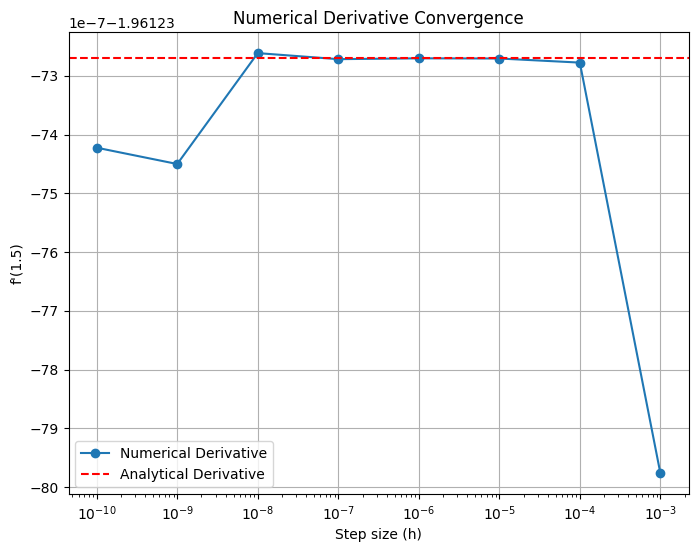
\includegraphics[scale=0.75]{task5plot.png}
\end{center}
It can be seen that the \textbf{numerical derivative} converge at all the steps between \texttt{1e-8} and \texttt{1e-5} but diverge at very small step sizes or very large step sizes. This means that \textbf{numerical derivative} only gives us stability and accuracy in a specific range of step sizes hence that it is very sensitive to step-size selection. The sensitivity comes from the fact that at very small $h$, rounding errors dominate due to floating-point precision limitations. Conversely, at large $h$, truncation error increases because the approximation becomes less accurate.

This does not apply to dual numbers as it does not depend on step size. The derivative is computed exactly using algebraic properties. A dual number \(x = a + b\epsilon\) automatically propagates both the value of \(f(a)\) and the derivative \(f'(a)\) when passed through a function \(f(x)\). Hence it eliminates all approximation errors that happen during numerical differentiation. Dual numbers also compute the derivative in a \textbf{single pass} through the function, which is more efficient.

\newpage
\section{Building the test suite (task 6)}
Many errors can arise when running any Python package. To make sure that the code is error-free and robust, the best way is to write a test suite to check every functionality of the package every time we update its distribution. The way we develop the test suite is, firstly, to check whether all of the codes we implement in \texttt{Dual} give us the expected answers, and also think of any possible edge cases cases.

In the package file \texttt{dual\_autodiff}, we have one \texttt{\_\_init\_\_.py} file and one module (\texttt{.py} files). \texttt{dual.py} is the main \texttt{Dual} class where we implement the core functionality like mathematical operations. We also add an extended definitions for the \texttt{Dual} class, where we define functions to simplify and accelerate computations for more complex functions such as \(tanh\).

Accordingly, in the test file, we want to a file corresponding to these modules called \texttt{autodiff\_tools.py}. This file provides all test cases for the \texttt{dual.py} module, focusing on special cases.

The first thing we want to test is whether the function is correct. We want to have examples and use \texttt{assert} to check whether the package result in the answer that we expected.

Next, there are several types of errors, however, because of the nature of the module, we may only encounter \texttt{ZeroDivisionError}, \texttt{TypeError}, \texttt{ValueError} and \texttt{AttributeError}. Since we want accuracy in the package, there is no Exception handling.

\texttt{TypeError} occurs when an operation or function is applied to an object of inappropriate type. For example, 
\begin{lstlisting}
    def test_initialization_with_non_numeric_real():
    with pytest.raises(TypeError):
        Dual("two", 1)
\end{lstlisting}
\texttt{ZeroDivisionError} happens when attempting to divide by zero. For example,
\begin{lstlisting}
    def test_division():
    x = Dual(6, 2)

    # Division by Dual with zero real part (raises error)
    with pytest.raises(ZeroDivisionError):
        x / Dual(0, 0)
\end{lstlisting}
Last but not least, \texttt{AttributeError} raised when an attribute referenced is unavailable, i.e, not defined in the package. An example of it is
\begin{lstlisting}
    def test_attribute_error_on_nonexistent_attribute():
    x = Dual(2, 1)
    with pytest.raises(AttributeError):
        value = x.non_existent_attribute
\end{lstlisting}

With more than 20 tests conducted, the \texttt{dual.py} file is verified and implements all necessary mathematical concepts and the package can be used confidently.

\section{Documentation with Sphinx (task 7)}
The objective of this task was to develop comprehensive and user-friendly documentation for the \texttt{dual\_autodiff} Python package using Sphinx \cite{sphinx}. The documentation is intended to assist users in understanding and using the package effectively by providing clear explanations, detailed examples, and interactive tutorials.

These are the steps that we need to make:
\subsection*{Sphinx Setup}

The \texttt{docs} directory contains a basic Sphinx configuration that was generated using:

\begin{lstlisting}[language=bash]
sphinx-quickstart
\end{lstlisting}

This initial setup created essential files such as \texttt{conf.py}, \texttt{index.rst}, and a \texttt{Makefile}.

\subsection*{Integration with Code and Notebooks}

\paragraph{Docstrings:} The documentation is built directly from Python docstrings. We follow Google-style docstring conventions, the codebase's function and class descriptions are automatically pulled into the documentation.

\paragraph{Tutorial Notebook:} A Jupyter notebook named \texttt{TutorialNotebook.ipynb} is included in the \texttt{docs} folder. This notebook provides a hands-on tutorial, guiding new users through the functionalities of the \texttt{dual\_autodiff} package. It includes:
\begin{itemize}
    \item \textbf{Introduction:} Introduce the concept of Dual numbers and why the package is needed in the modern world.
    \item \textbf{Explanations:} Clear textual explanations accompany the code to ensure that users understand what the library does and how to apply it to their own problems.
    \item \textbf{Code Snippets:} Step-by-step examples on how to instantiate dual numbers and apply forwardmode differentiation.
    \item \textbf{Examples:} Demonstrations of how to perform automatic differentiation on various mathematical functions.
\end{itemize}

\subsection*{Building the Documentation}

To generate the HTML documentation, simply run:

\begin{lstlisting}[language=bash]
cd docs
make html
\end{lstlisting}

This command processes the \texttt{index.rst}, imports docstrings from the \texttt{dual\_autodiff} codebase. We also added two \texttt{.rst} files, one is \texttt{tutorials.rst} to read the Jupyter notebook and the other \texttt{api\_reference.rst} to read the API. The resulting HTML files are placed in \texttt{docs/\_build/html}, ready to be opened in a browser.

\subsection*{Outcome}

The final documentation site provides:
\begin{itemize}
    \item A clean index page that introduces \texttt{dual\_autodiff}.
    \item API documentation automatically generated from the codebase's docstrings, ensuring accuracy and up-to-date information.
    \item A tutorial notebook that illustrates practical use cases, helping users quickly grasp the core functionalities of the package.
\end{itemize}

By integrating docstrings with Sphinx and providing a user-friendly notebook tutorial, the \texttt{dual\_autodiff} documentation ensures that both new and experienced users can understand the project's purpose, capabilities, and intended usage patterns.

\newpage

\section{Cython and performance comparison (task 8+9)}
\subsection{Cythonize pure Python}
The core code consists of these following files: 
\vspace{0.5cm}
\dirtree{%
    .1 pyproject.toml. % Project configuration file.
    .1 dual\_autodiff/.      
    .2 \_\_init\_\_.py. % Makes it a Python package.
    .2 autodiff\_tools.py.
}
\vspace{0.5cm} 
To cythonize the package \texttt{dual\_autodiff}, we follow the steps as stated in the lecture notes:
\begin{enumerate}
    \item Move the python files into a \texttt{/dual\_autodiff\_x} folder.
    \item Rename the \texttt{.py} files into \texttt{.pyx} files.
    \item Modify the \texttt{pyproject.toml} file and add \texttt{setup.py} file.
\end{enumerate}

Then from the inside the folder we can install \texttt{dual\_autodiff\_x} by using the line 
\newline \texttt{python setup.py build\_ext --inplace}. The hardest part of the task is modifying the \texttt{setup.py} file because we want to know the package structure and repository well to create the correct setup.

\subsection{Performance Comparision}
We want to analyse the difference in performance of the Dual number class using \textbf{pure Python version} (\texttt{dual\_autodiff.dual}) and the \texttt{Cythonized version} (\texttt{dual\_autodiff.dual.dual}). From here we can make up our mind of which version to choose when it comes to optimisation and computational efficiency.

\subsubsection{Steps}
\begin{enumerate}
    \item Implementations:
    \begin{itemize}
        \item Pure Python version of the Dual class is implemented using standard Python constructs. It includes methods for basic arithmetic operations, leveraging Python's dynamic typing and interpreted nature.
        \item Cythonized version translates the Dual class into Cython with optional, C-inspired syntax extensions that yields performance comparable to C.
        \item Both of the implementations were tested within the same file \texttt{dual\_autodiff.ipynb} to ensure fairness and on MacBook Air with Apple M1 chip running Python 3.9.
    \end{itemize}


    \item Performance measurement: generating 2 test functions to perform arithmetic operations (addition and multiplication). The \texttt{timeit} module was used to measure the execution time of both functions in many numbers of operations \texttt{n}: 1,000; 5,000; 10,000; 50,000; 100,000; 500,000. Each test was run multiple times to obtain average execution times, ensuring statistical reliability.

    \item Data visualisation : execution time was plotted using \texttt{matplotlib} to visually compare performance.
\end{enumerate}

\subsubsection{Results}
This table and plot below summarise the execution time for both implementations.
\begin{table}[h!]
\centering
\caption{Execution Times and Speedup Factors}
\label{tab:execution_times}
\begin{tabular}{|c|c|c|c|}
\hline
\textbf{Number of Operations (n)} & \textbf{Pure Python Time (s)} & \textbf{Cythonized Time (s)} & \textbf{Speedup Factor} \\ \hline
1,000 & 0.0115 & 0.0046 & 2.47× faster \\ \hline
5,000 & 0.0591 & 0.0415 & 1.42× faster \\ \hline
10,000 & 0.2274 & 0.0687 & 3.31× faster \\ \hline
50,000 & 0.4178 & 0.1646 & 2.54× faster \\ \hline
100,000 & 0.7642 & 0.5241 & 1.46× faster \\ \hline
500,000 & 4.1356 & 1.7390 & 2.38× faster \\ \hline
\end{tabular}
\end{table}
\begin{center}
    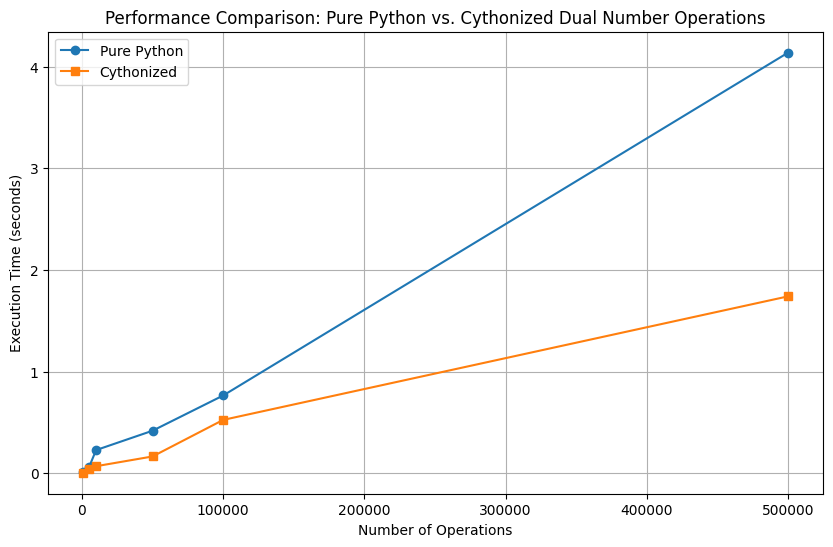
\includegraphics[scale=0.75]{task9.png}
\end{center}

Across all tested operation counts, the Cythonized implementation outperformed the pure Python version, achieving speedup factors ranging from 1.42× to 3.31× faster. In simple operations like addition or a small number of multiplications, Python's overhead is not as significant relative to the actual computation. Hence, the speedup from Cython is smaller. For computationally expensive operations (e.g., large loops or repeated calculations), Cython has significant speedups.

The significant performance gains observed in the Cythonized implementation can be attributed to several factors:
\begin{itemize}
    \item Cython allows for better management of how memory is used, helping the CPU access data more quickly and reducing delays.
    \item By turning Python code into C, Cython removes the slow step of interpreting code, making the program run faster, especially in loops that perform many calculations. \cite{wilbers2009using}
\end{itemize}
\newpage
\section{Linux Wheel Creation with \texttt{cibuildwheel} (task 10)}

\subsection*{Create Wheels}

To generate Linux wheels for \texttt{dual\_autodiff\_x}, we used \texttt{cibuildwheel} \cite{cibuild}, which employs Docker to create portable and compliant binary distributions. The objective was to build wheels for the following environments:

\begin{itemize}
    \item Python 3.10 on \texttt{manylinux\_x86\_64} (i.e., \texttt{cp310-manylinux\_x86\_64})
    \item Python 3.11 on \texttt{manylinux\_x86\_64} (i.e., \texttt{cp311-manylinux\_x86\_64})
\end{itemize}

We build the wheels by running \texttt{cibuildwheel} with the appropriate configuration (such as specifying the \texttt{CIBW\_ARCHS} and \texttt{CIBW\_MANYLINUX\_X86\_64\_IMAGE} environment variables), 

\begin{lstlisting}[frame=single]
export CIBW_BUILD="cp310-manylinux_x86_64 cp311-manylinux_x86_64"
export CIBW_ARCHS=x86_64
cibuildwheel --platform linux
\end{lstlisting}

we obtained the following wheels in the \texttt{wheelhouse} directory:

\begin{lstlisting}[frame=single]
dual_autodiff_x-0.0.1b2-cp310-cp310-manylinux_2_17_x86_64.manylinux2014_x86_64.whl
dual_autodiff_x-0.0.1b2-cp311-cp311-manylinux_2_17_x86_64.manylinux2014_x86_64.whl
\end{lstlisting}

These wheels were successfully built, we make to make sure the build configuration and the correct Docker images and environment variables are set accordingly. 

\subsection*{Verification of Wheel Contents}

To confirm that the wheels do not contain the original \texttt{.pyx} source code files, but only the compiled \texttt{.so} (and \texttt{.pyd} on other platforms) files, the following steps were taken:

\begin{enumerate}
    \item Extract the wheel's contents:
    \begin{lstlisting}[language=bash]
    unzip dual_autodiff_x-0.0.1b2-cp310-cp310-manylinux_2_17_x86_64.manylinux2014_x86_64.whl -d wheel_contents
    unzip dual_autodiff_x-0.0.1b2-cp311-cp311-manylinux_2_17_x86_64.manylinux2014_x86_64.whl -d wheel_contents\end{lstlisting}
    
    \item Inspect the \texttt{wheel\_contents} directory to ensure it contains only the expected binary files.
\end{enumerate}

The desired final state is to produce two wheels that include only the compiled binary artifacts. Adjusting the \texttt{cibuildwheel} configuration to target the \texttt{x86\_64} architecture and verifying the file contents as described above ensures compliance with the specified requirements.

\section{Uploading Wheels to GitLab and Verifying Installation (task 11)}

After building the required Linux-compatible wheels for the \texttt{dual\_autodiff\_x} package, these wheels were uploaded to the project's GitLab repository. Storing pre-compiled wheels in a  repository ensures ease of access and eliminates the need for source compilation on end-user machines.

\subsection{Procedure}

\begin{enumerate}
    \item \textbf{Wheel Creation:} The wheels were generated using \texttt{cibuildwheel}, which runs in a Docker environment. This ensures that the final wheels comply with the \texttt{manylinux} specifications and are fully portable.
    
    \item \textbf{Uploading to GitLab:} Once generated, the wheel files were uploaded directly to the GitLab project repository, under \texttt{dual\_autodiff\_x/wheelhouse} directory. This makes the wheels easily accessible to collaborators and end-users.
    
    \item \textbf{Verification of Installation:} To confirm that the wheels work as intended, they were downloaded from the GitLab repository onto the Docker Desktop and installed using:
    \begin{verbatim}
    docker build --platform linux/amd64 -t my-python-app .
    docker run -p 8888:8888 my-python-app      
    \end{verbatim}
\end{enumerate}

\subsection{Testing the Installation}

After installing the wheel, the \texttt{dual\_autodiff\_x} package was tested by running the provided examples in the tutorial notebook (i.e., \texttt{TutorialNotebook\_x.ipynb}). The code executed successfully, confirming that:

\begin{itemize}
    \item The wheels were properly built and require no additional compilation.
    \item Users can immediately utilize the package upon installation.
    \item The notebook examples ran smoothly, validating the integrity and functionality of the distributed wheels.
\end{itemize}

\subsection{Outcome}

By hosting the wheels in the GitLab repository, the distribution and installation process is significantly simplified. Users can simply download and install the pre-built wheels, thus avoiding common build-related complications. This approach ensures a more user-friendly and robust installation experience, allowing researchers and practitioners to focus on leveraging the \texttt{dual\_autodiff\_x} library’s capabilities rather than dealing with installation hurdles.


\addcontentsline{toc}{section}{Bibliography} 

\bibliographystyle{ieeetr}
\bibliography{reference}

Word count : 2787
\end{document}
